\documentclass[
  11pt,
  letterpaper,
   addpoints,
   answers
  ]{exam}

\usepackage{../exercise-preamble}

\begin{document}

\noindent
\begin{minipage}{0.47\textwidth}

\includegraphics[width=\textwidth]{../fcfm_die}
\end{minipage}
\begin{minipage}{0.53\textwidth}
\begin{center} 
\large\textbf{Electromagnetismo Aplicado} (EL3103-1) \\
\large\textbf{Clase auxiliar 4} \\
\normalsize Prof.~Benjamin Jacard H.\\
\normalsize Prof.~Aux.~Erik Saez A.
\end{center}
\end{minipage}

\vspace{0.5cm}
\noindent
\vspace{.85cm}

\begin{questions}
    %%%%%%%%%%%%%%%%%%%%%%%%%%%%
    \question En el toroide delgado de la figura, determinar:

    \begin{enumerate}
        \item La impedancia del enrollado de $N$ vueltas en primera aproximación (despreciando energía almacenada en campo eléctrico).
        \item El campo eléctrico fasorial de mayor amplitud en el entrehierro.
    \end{enumerate}
    
    \textbf{Nota}: Suponga que el campo magnético en el toroide es uniforme e igual al correspondiente al radio medio. Despreciar efectos de borde y pérdidas.
    \begin{center}
        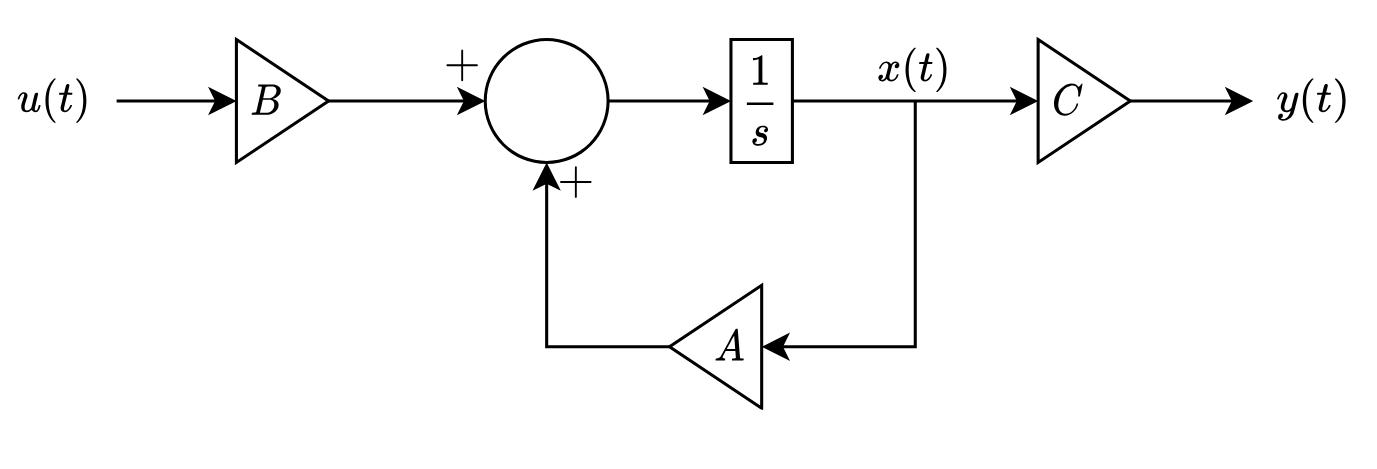
\includegraphics[width=0.4\textwidth]{Auxiliar_4_1}
        \captionof{figure}{Esquema del toroide}
      \end{center}
    %%%%%%%%%%%%%%%%%%%%%%%%%%%%
    \begin{solution}
        \begin{enumerate}
            \item Se busca obtener la impedancia del enrollado despreciando la energia almacenada en el campo electrico, por lo que se tiene que:
       \begin{equation}
        Z= jwL = j \frac{4\omega}{|I_{0}|^{2}}<W_{m}>
       \end{equation}
       Utilizando la forma integral de la ley de Ampere se tiene que:
       \begin{align}
        \oint_C \vec{H} \cdot d\vec{l} &= N I_0 e^{j\omega t}
       \end{align}
       Consideramos el radio medio del toroide, el cual podemos ver que 
       se define como:
    \begin{equation}
        r_m = \frac{a + b}{2}
    \end{equation}  
    Aplicando la ley de Ampère:
    \begin{equation}
    \oint_C \vec{H} \cdot d\vec{l} = H_1(2\pi r_m - g) + H_2 g = N I_0 e^{j\omega t}
    \end{equation}
     Dado que por condicion de borde se debe cumplir \( B_1 = B_2 \Rightarrow \mu H_1 = \mu_0 H_2 \), se obtiene:
    \begin{equation}
        \frac{\mu_0}{\mu} H_2 (2\pi r_m - g) + H_2 g = N I_0 e^{j\omega t}
    \end{equation}

Despejando \( H_2 \):
\begin{equation}
H_2 = \frac{\mu N I_0}{\mu_0 (2\pi r_m - g) + \mu g}
\end{equation}

De manera análoga podemos despejar \( H_1 \) dando como resultado:
\begin{equation}
H_1 = \frac{\mu_0 N I_0}{\mu_0 (2\pi r_m - g) + \mu g}
\end{equation}
Dado que despreciamos la energia almacenada en el campo electrico, nos centraremos unicamente en la energia almacenada en el campo magnetico, por lo que se tiene que:
\begin{equation}
\frac{1}{4} L I_0^2 = \frac{1}{4} \int_{\text{vol toroide}} \vec{B} \cdot \vec{H^{*}} \, dv
\end{equation}

La cual puede expresarse como:
\begin{align}
\frac{1}{4} L I_0^2 &= \frac{1}{4} \mu H_1^2 \cdot \frac{\pi (b - a)^2}{4} \cdot (2\pi r_m - g) + \frac{1}{4} \mu_0 H_2^2 \cdot \frac{\pi (b - a)^2}{4} \cdot g \\
\frac{1}{4} L I_0^2 &= \frac{1}{4} \mu \left( \frac{\mu_0 N I_0}{\mu_0(2\pi r_m - g) + \mu g} \right)^2 \cdot \frac{\pi (b - a)^2}{4} \cdot (2\pi r_m - g) \notag \\
&\quad + \frac{1}{4} \mu_0 \left( \frac{\mu N I_0}{\mu_0(2\pi r_m - g) + \mu g} \right)^2 \cdot \frac{\pi (b - a)^2}{4} \cdot g
\end{align}
Factorizando y despejando \( L \):
\begin{equation}
L = \frac{N^2 \pi (b - a)^2}{4 \left[ \mu_0(2\pi r_m - g) + \mu g \right]^2} \left[ \mu \mu_0 (2\pi r_m - g) + \mu_0^2 g \right]
\end{equation}

\begin{equation}
L = \frac{N^2 \pi (b - a)^2 \mu \mu_0}{4 \left[ \mu_0(2\pi r_m - g) + \mu g \right]}
\end{equation}
De esta manera es posible obtener la impedancia buscada en el problema.
   
\item Luego se busca obtener el campo electrico en el entrehierro por lo que aplicando la ley de inducción de Faraday, la cual se deriva a partir de lo siguiente:
\begin{align}
    \nabla \times \vec{E} &= -\frac{\partial \vec{B}}{\partial t} \\
\end{align}
Escrita en su forma integral se tiene que:
\begin{align}
    \oint_C \vec{E} \cdot d\vec{l} &= -\frac{d}{dt} \int_S \vec{B} \cdot d\vec{S}
\end{align}
De esta manera en notacion fasorial tenemos la notacion dada por:
\begin{equation}
\oint_C \vec{E} \cdot d\vec{l} = -j \omega \psi
\end{equation}

\noindent
Donde \( \psi \) es el flujo magnético, y se cumple:
\begin{equation}
E(r) \cdot 2\pi r = -j\omega \int_S \mu_0 H_2 \, ds
\end{equation}
Siendo \( S \) la sección transversal de radio \( r \), y considerando que \( H_2 \) es constante en dicha superficie:

\begin{equation}
E(r) \cdot 2\pi r = -j\omega \mu_0 H_2 \cdot \pi r^2
\end{equation}

Despejando \( E(r) \):

\begin{align}
E(r) &= -j\omega \frac{\mu_0}{2} r H_2 \\
&= -j\omega \frac{\mu_0}{2} r \cdot \frac{\mu N I_0}{\mu_0(2\pi r_m - g) + \mu g}
\end{align}

Finalmente, se observa que el campo eléctrico es máximo para:
\begin{equation}
r = \frac{b - a}{2}
\end{equation}

\end{enumerate}
    \end{solution}
    %%%%%%%%%%%%%%%%%%%%%%%%%%%%
    \question  Considere un condensador con electrodos circulares, entre los electrodos existe una diferencia de potencial
    v(t).
    \begin{enumerate}
        \item Determine el campo eléctrico y el campo magnético al interior del condensador (asuma dieléctrico con $\epsilon_{0}, \mu_{0}$)
        \item Calcule el vector de Poynting. ¿Que dirección tiene?
        \item  Calcule la tasa de cambio de la energia al interior del condensador, usando el vector de Poynting.
        \item Compare la respuesta anterior calculando la tasa de cambio de la energia eléctrica almacenada por el
    condensador.
    \begin{center}
        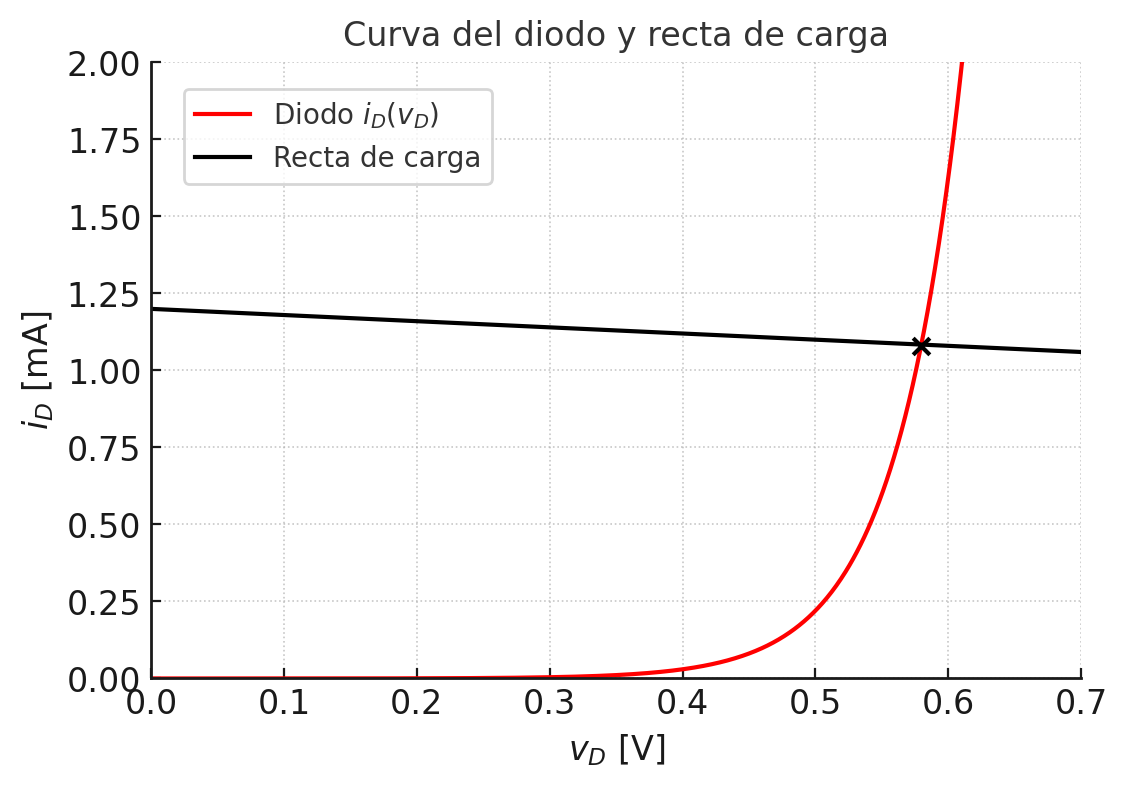
\includegraphics[width=0.4\textwidth]{Auxiliar_4_2}
        \captionof{figure}{Esquema del toroide}
      \end{center}
    \end{enumerate}
    %%%%%%%%%%%%%%%%%%%%%%%%%%%%
    \begin{solution}
         \begin{enumerate}
            \item Se busca el obtener el campo eléctrico y magnético del condensador el cual posee un \textbf{Campo variable en el tiempo} , que es importante a tener en cuenta.\\
            \subsubsection*{\underline{Campo eléctrico}}
            Este se obtendrá de manera directa:
            \begin{align}
                V(b) - V(a) &= - \int^{b}_{a} E(t)\cdot dl (\hat{z} 
             \cdot \hat{z})\\
            \end{align}
            Se puede observar que  V(b) - V(a) sera equivalente a v(t) dado que representa los terminales del capacitador y este varia en todo momento.
            \begin{align}
                V(t) &= E(t) d\\
                E(t) &= \frac{V(t)}{d}\hat{z}
            \end{align}
            \subsubsection*{\underline{Campo magnético}}
            Sabemos por ley de Ampere que se tiene lo siguiente:
            \begin{align}
                \nabla \times H = J + \frac{\partial D}{\partial t}
            \end{align}
            Se tiene que J=0 debido a que en el espacio del condensador no existe una densidad de carga y tampoco una corriente ``real''. pero  si se considera el termino de corrección(\textit{Es decir el desplazamiento}).
            \begin{align}
                \nabla \times H &= \frac{\partial D}{\partial t}\\
                                &= \epsilon \frac{\partial E(t)}{\partial t}\\
                                &= \frac{\epsilon}{d}\frac{\partial V(t)}{\partial t}
            \end{align}
            Luego en su forma diferencial se tendrá que:
            \begin{align}
                \int H \cdot dl = \frac{\epsilon}{d}\int \frac{\partial V(t)}{\partial t} \cdot dS
            \end{align}
            Debido a la geometría y teniendo en cuenta que H envolverá al campo eléctrico \textit{(Regla de la mano derecha)}, se tendrá lo siguiente:
            \begin{align}
                H (2\pi r) &= \frac{\epsilon}{d} \frac{\partial V}{\partial t} \pi r^{2}\\
                H &= \frac{\epsilon r}{2d} \frac{\partial V}{\partial t} \hat{\theta}
            \end{align}
            \item Se tiene que el vector de Poynting viene dado por $\hat{S} = \hat{E} \times \hat{H}$, el cual es un vector perpendicular tanto para el campo eléctrico como magnético y este nos da la dirección y magnitud del flujo de energía electromagnética.\href{http://jnaudin.free.fr/html/pft01.htm}{(\textcolor{magenta}{Idea visual})}
            \begin{align}
                \hat{S} = \hat{E} \times \hat{H} &= \left(\frac{V(t)}{d}\right) \hat{z} \times \left(\frac{\epsilon r}{2d}\frac{\partial V(t)}{\partial t}\right) \hat{\theta}\\
                &= \frac{\epsilon r}{2d^{2}} V(t) \left(\frac{\partial V(t)}{\partial t}\right) (\hat{z} \cdot \hat{\theta})\\
                &= - \frac{\epsilon r}{2d^{2}} V(t) \left(\frac{\partial V(t)}{\partial t}\right) \hat{r}
            \end{align}
            \item Tal de profundizar con respecto al vector de Poynting, se realiza las siguientes relaciones mediantes las ecuaciones de Maxwell,
            {\small
            \begin{align}
               H\cdot (\nabla \times E ) - E \cdot (\nabla \times H) &= \nabla \cdot (E \times H)\\
               -H \cdot \frac{\partial B}{\partial t} - E \cdot \frac{\partial D}{\partial t} - E \cdot J  &=  \nabla \cdot (E \times H)\\
               \int_{V} \left( -H \cdot \frac{\partial B}{\partial t} - E \cdot \frac{\partial D}{\partial t} - E \cdot J \right) dv &= \int_{V} \left( \nabla \cdot (E \times H) \right) dv\\
               \int_{V} \left( H \cdot \frac{\partial B}{\partial t} + E \cdot \frac{\partial D}{\partial t}+ E \cdot J \right) dv &= -\oint_S \left(E \times H \right) ds
            \end{align}
            }
            Descompuesta de esta manera el vector de Poynting permite realizar el siguiente análisis:
            \begin{itemize}
                \item $H \cdot \frac{\partial B}{\partial t}$ : Corresponde a la energía magnética almacenada 
                \item $E \cdot \frac{\partial D}{\partial t}$ : Corresponde a la energía eléctrica almacenada
                \item $ E \cdot J $ Corresponde a la energía disipada por calor ``Ohmica''
            \end{itemize}
            Por lo tanto $\oint_S \left(E \times H \right) ds$ da cuenta de la variación de la energía almacenada en el condensador con respecto al tiempo . Luego lo calculamos sobre la superficie que nos interesa (\textit{Superficie entre placas}) obteniendo lo siguiente:
            {\small
            \begin{align}
                -\oint_{S} (E\times H)ds |_{r=b} &= -\int_{0}^{d} \int_{0}^{2\pi} -\frac{\epsilon b}{2d^{2}}V(t) \left(\frac{\partial V(t)}{\partial t} \right) b (d\phi)(dz) (\hat{r} \cdot \hat{z})
            \end{align}}
            \begin{align}
                &=  -\frac{\epsilon b^{2}}{2d^{2}}V(t) \left(\frac{\partial V(t)}{\partial t}\right) \cdot 2\pi d (-\hat{\theta})\\
                &=  -\frac{\epsilon \pi b^{2}}{d}V(t) \left(\frac{\partial V(t)}{\partial t}\right)(-\hat{\theta})\\
                &= \frac{1}{2} \frac{\epsilon b^{2} \pi}{ d} \cdot \frac{\partial (V(t))^{2}}{\partial t}(\hat{\theta})\\
                &= \frac{\partial}{\partial t} \left( \frac{1}{2} CV^{2}\right)(\hat{\theta})
            \end{align}
            (Se utilizo que  $V(t) \left(\frac{\partial V(t)}{\partial t}\right)  = \frac{\partial}{\partial t} (\frac{1}{2} V(t)^{2})$). Finalmente se observa que depende solo de la variación de la energía eléctrica almacenada, lo cual concuerda de buena manera con el hecho de que estamos trabajando con un condensador.\item Se busca obtener el cambio de la energía eléctrica almacenada por el condensador, lo cual utilizando la expresión conocida de energía almacenada tenemos que:
            \begin{align}
                W_{e} &= \frac{\partial}{\partial t} \int_{V} \frac{1}{2} \epsilon \|E\|^{2} dV\\
                      &= \frac{\partial}{\partial t} \int_{V} \frac{1}{2} \epsilon \frac{V(t)^{2}}{d^{2}} dV\\
                      &= \frac{\partial}{\partial t} \left( \frac{\epsilon V(t) ^{2}}{2d^{2}}\right) \int dV\\
                      &= \frac{\partial}{\partial t} \left( \frac{\epsilon V(t) ^{2}}{2d^{2}}\right) \cdot \pi b^{2} d\\
                      &= \frac{\partial}{\partial t} \left(\frac{\epsilon V(t)^{2} \pi b^{2}}{2d}\right)\\
                      &= \frac{\partial}{\partial t} \left( \frac{1}{2} CV(t)\right)
            \end{align}
            Notar la relación con lo obtenido en la parte c) , esto nos quiere decir que la variación de la energía total depende por tanto solo del \textbf{campo eléctrico}
            \item Se tiene que toda la energía almacenada en el condensador es puramente eléctrica y esto es debido al funcionamiento perse de un condensador, dado que este almacena dicha energía dentro de sus placas debido a la corriente de desplazamiento, análisis similiar que se puede realizar para una inductancia.
         \end{enumerate}
    \end{solution}
    %%%%%%%%%%%%%%%%%%%%%%%%%%%
    \question  Considere una linea de transmisión cuya sección trasversal se muestra en la figura. Suponga que se propaga una onda transversal electromagnética según z+, donde $V_{0}$ es el valor máximo del voltaje. Se considera un dieléctrico perfecto es decir $\sigma = \infty$.
    \begin{enumerate}
        \item Potencial $\phi(r, \theta)$ para a $\leq$ r $\leq$ b
        \item Campo eléctrico fasor $E(r, \theta, z, t)$
        \item Densidad de corriente $J_{s}$ y corriente total en los conductores (r=a) y (r=b)
        \item Potencia media transmitida $< P_{t} >$ en base al vector de Poynting.
        \item  Energıa almacenada en campo eléctrico $< W_{e} >$ y campo magnético $< W_{m} >$ , por unidad de longitud de la linea
    \end{enumerate}
    \begin{center}
        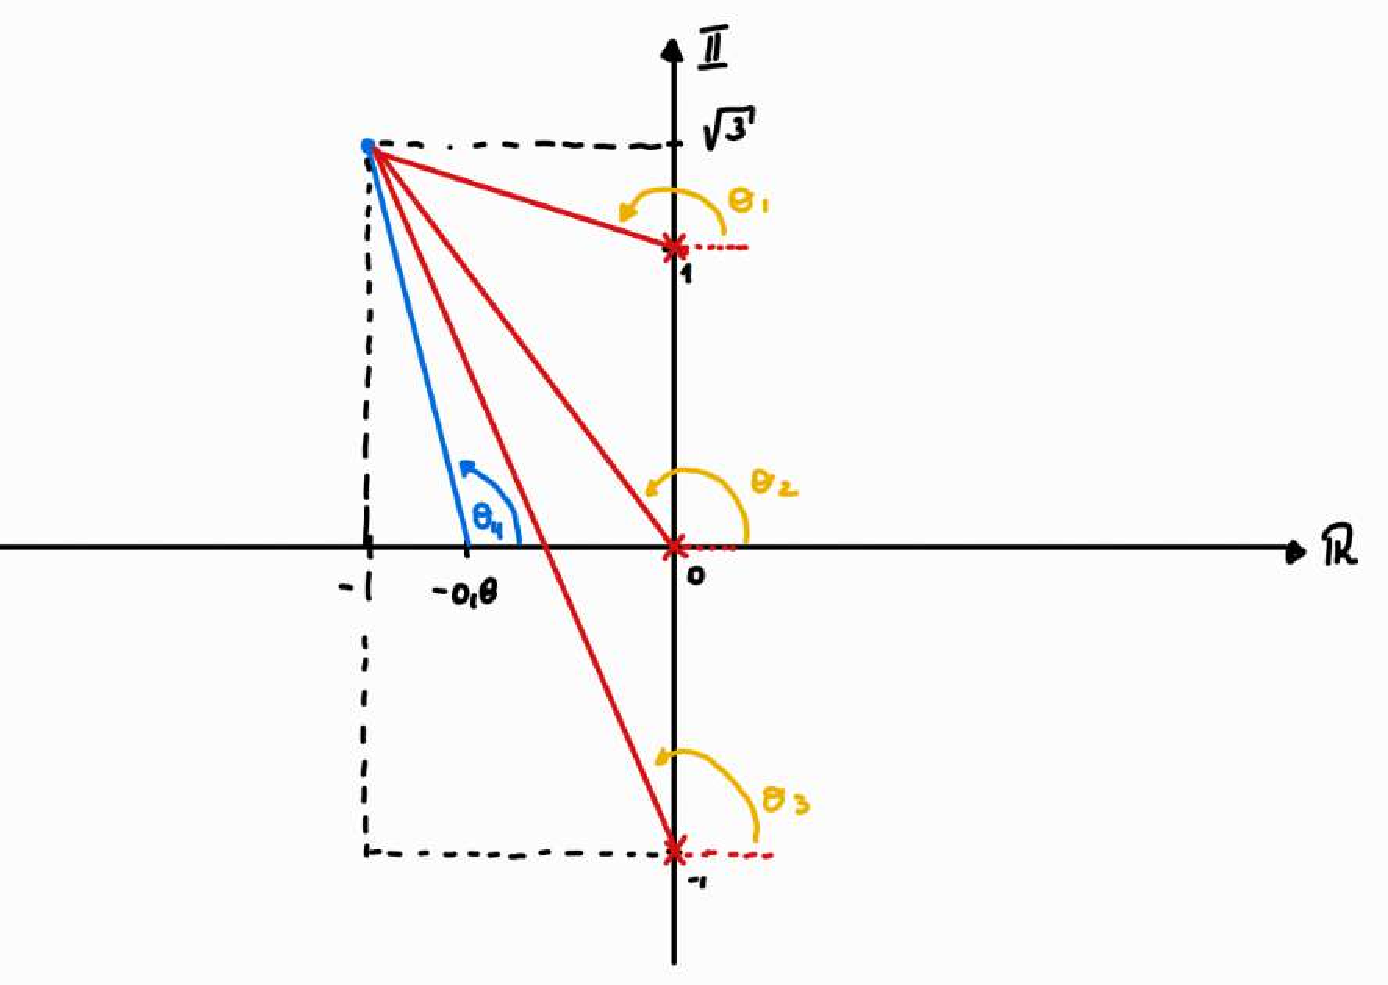
\includegraphics[width=0.4\textwidth]{Auxiliar_4_3}
        \captionof{figure}{Esquema del toroide}
      \end{center}
    %%%%%%%%%%%%%%%%%%%%%%%%%%%
    \begin{solution}
        \begin{enumerate}
            \item Se busca obtener el potencial eléctrico $\phi(r,\theta)$ para (a $\leq$ r $\leq$ b) , por lo que se utilizara  coordenadas cilíndricas y dada la distribución de las placas se tendrá solo dependencia en r:
            \begin{align}
                \nabla^{2}\phi(r,\theta) =\frac{1}{r} \frac{\partial}{\partial r}\left(r \frac{\partial \phi}{\partial r}\right)= 0
            \end{align}
            Luego integrando sigue que:
            \begin{align}
                \frac{1}{r} \frac{\partial}{\partial r}\left(r \frac{\partial \phi}{\partial r}\right)&= 0\\
                 \frac{\partial}{\partial r}\left(r \frac{\partial \phi}{\partial r}\right)&= 0\\
                 \left(r \frac{\partial \phi}{\partial r}\right)&= A\\
                 \frac{\partial \phi}{ \partial r} =& \frac{A}{r}\\
                 \phi(r) =& Aln(r) + B
            \end{align}
            Con lo que se obtiene la forma del expresión del potencial. Luego se deberá obtener las constantes mediante las condiciones de borde para obtener una expresión particular.
            \begin{align}
                \phi(r=a) = V_{0}e^{jwt}= Aln(a)+ B
            \end{align}
            Mientras que por otro lado
            \begin{align}
                \phi(r=b)= 0 = Aln(b) + B\\
                B= -Aln(b)
            \end{align}
            Reemplazando este ultimo:
            \begin{align}
                V_{0}e^{jwt}&= Aln(a)- Aln(b)\\
                A &= \frac{V_{0}e^{jwt}}{ln(\frac{a}{b})}
            \end{align}
            Finalmente se tendrá que:
            \begin{align}
                \phi(r) = \frac{V_{0}e^{jwt}}{ln(\frac{a}{b})} ln(r)-\frac{V_{0}e^{jwt}}{ln(\frac{a}{b})}ln(b)
            \end{align}
            \item Se busca obtener una expresión para el campo eléctrico, por lo que tenemos:
            \begin{align}
                E(r,\theta,z,t) &= -\nabla\phi(r) = - \frac{\partial}{\partial r} \left(\frac{V_{0}e^{jwt}}{ln(\frac{a}{b})} ln(r)-\frac{V_{0}e^{jwt}}{ln(\frac{a}{b})}ln(b)\right)\\
                &= \frac{V_{0}e^{jwt}}{ln(\frac{a}{b})} \frac{1}{r}(\hat{r})
            \end{align}
            Es importante considerar que el campo eléctrico se propaga como una onda transversal electromagnética por lo que debemos añadir dicha componente por lo tanto,
            \begin{align}
                E(r,\theta,z,t)= \frac{V_{0}}{ln(a/b)} \frac{1}{r} e^{-jbz}e^{jwt}(\hat{r})
            \end{align}
            Es importante tener en cuenta que estamos considerando el caso sin perdidas, es por esto que no existe la presencia de un ($\alpha$) (\textit{Se vera en la siguiente unidad como interpretar esto})
\item Se busca obtener la densidad de corriente superficial $J_{s}$ y la corriente total en los conductores 
(r=a) y (r=b). Dada la presencia de una pared eléctrica con conductividad infinita, se considera que toda la intensidad magnético se relaciona de la siguiente manera con la densidad de corriente superficial 
\begin{align}
    \hat{n} \times H = J_{s}
\end{align}
Por tanto se utiliza la siguiente expresión equivalente (\textit{Se evalúa el campo H dado que estamos considerando en una superficie en particular}):
\begin{align}
    J_{s}= \hat{n} \times H(r=a)
\end{align}
Se puede relacionar el campo eléctrico y magnético: (\textit{El termino Y corresponde a la admitancia del medio}):
\begin{align}
    H_{1}(r=a) &= Y(\hat{k}) \times E(r=a) (\hat{r})\\ H_{1}(r=a) &= \frac{Y V_{0}}{ln(a/b)} \frac{1}{a} e^{-jbz}e^{jwt}(\hat{\theta})
\end{align}
Por lo que finalmente se tendrá que:
\begin{align}
    J_{s}(r=a)&= (\hat{r}) \times H_{1}(r=a) (\hat{\theta})  \\
     &= \frac{Y V_{0}}{ln(a/b)} \frac{1}{a} e^{-jbz}e^{jwt}\hat{\theta}(\hat{r} \times \hat{\theta}) \\
     &= \frac{YV_{0}}{ln(a/b)} \frac{1}{a} e^{-jbz}e^{jwt}(\hat{k})
\end{align}
Lo cual es consistente dado que la corriente fluye hacia la pantalla. De manera análoga tenemos que para $J_{s}(r=b)$,
\begin{align}
    J_{s}(r=b) = (-\hat{r}) \times H(r=b) 
\end{align}
Se debe tener en consideración ese signo - dado la consistencia con la dirección, luego para  H(r=b):
\begin{align}
    H_{2}(r=b) &= Y\hat{k} \times E(r=b)\hat{r}\\
    &= Y \cdot \frac{V_{0}}{ln(a/b)} \frac{1}{b} e^{-jbz}e^{jwt}\hat{\theta}
\end{align}
Con lo que finalmente,
\begin{align}
    J_{s}(r=b) &= (-\hat{r}) \times H(r=b) \\
               &=  (-\hat{r}) \times Y \cdot \frac{V_{0}}{ln(a/b)} \frac{1}{b} e^{-jbz}e^{jwt}\hat{\theta}\\
               &= -\frac{YV_{0}}{b\cdot\
               ln(a/b)} e^{-jbz}e^{jwt} (\hat{k})
\end{align}
Con lo que se obtiene la densidad de corriente en ambas placas, finalmente se quiere obtener la corriente total en estas, por lo que:
\begin{align}
    I_{a} &= \int_{0}^{\theta_{0}} J_{s}(r=a) a(d\theta)\\
          &=\frac{YV_{0}}{ln(a/b)} \frac{1}{a} e^{-jbz}e^{jwt} \cdot (a\theta_{0})\\
          &= \frac{YV_{0}}{ln(a/b)}  e^{-jbz}e^{jwt} \cdot (\theta_{0})\
\end{align}
Por otro lado de manera análoga se tendrá que:
\begin{align}
    I_{b} &= \int_{0}^{\theta_{0}} J_{s}(r=b) b d(\theta)\\
          &= - \frac{YV_{0}}{ln(a/b)} \frac{1}{b} e^{-jbz}e^{jwt} \cdot (b\theta_{0})\\
          &= -\frac{YV_{0}}{ln(a/b)}  e^{-jbz}e^{jwt} \cdot (\theta_{0})\
\end{align}
Luego se observa que las corrientes en ambos medios es igual en magnitud pero con signos contrarios, lo cual es consistente con lo esperado.

\item Se busca obtener la potencia media transmitida $ \langle P_t \rangle $ en base al vector de Poynting:
\begin{align}
    \langle P_t \rangle = \int_{s} \frac{1}{2}Re(E \times H^{*}) dS
\end{align}
Reemplazando lo que ya obtuvimos con anterioridad,
\begin{align}
    \langle P_{t} \rangle &= \int_{s} \frac{1}{2}\operatorname{Re}(E \times H^{*}) \,dS\\
             &= \mbox{\small{$\operatorname{Re}\left( \frac{V_{0}}{\ln(a/b)} \frac{1}{r} e^{-jbz}e^{jwt}\hat{r} \times Y \cdot \frac{V_{0}}{\ln(a/b)} \frac{1}{r} e^{jbz}e^{-jwt}\hat{\theta} \right) \,dS$}}\\
             &= \frac{1}{2}\int_{s} \frac{V_{0}^{2}Y}{\ln(a/b)^{2}}\frac{1}{r^{2}} \,dS\\
             &= \frac{1}{2}\left(\frac{V_{0}}{\ln(a/b)}\right)^{2}Y \int_{0}^{\theta_{0}}\int_{a}^{b} \frac{r}{r^{2}} (\,dr)(\,d\theta)\\
             &= \frac{1}{2}\left(\frac{V_{0}}{\ln(a/b)}\right)^{2}Y \ln(a/b)\theta_{0}\\
             &= \frac{1}{2}\left(\frac{V_{0}^{2}}{\ln(a/b)}\right)Y \theta_{0}
\end{align}
Con lo que finalmente se obtiene la expresión planteada inicialmente.
\item Luego, queremos la energía almacenada en campo eléctrico $\langle W_{e} \rangle$ y campo magnético $\langle W_{m} \rangle$, por unidad de longitud de línea. Es por esto,
\begin{align}
    \langle W_{e} \rangle &= \int_{v} \frac{1}{4}\epsilon\|E\|^{2}(\,dv)\\
    &= \frac{\epsilon}{4}\int_{v}\|E\|^{2}(\,dv)\\
    &=\frac{\epsilon}{4}\int_{v} \left( \frac{V_{0}}{\ln(a/b)} \frac{1}{r}\right)^{2} r(\,dr)(\,d\theta)(\,dz)\\
    &= \frac{\epsilon}{4}\left( \frac{V_{0}}{\ln(a/b)}\right)^{2}\int_{v} \frac{r}{r^{2}}(\,dr)(\,d\theta)(\,dz)\\
    &= \frac{\epsilon V_{0}^{2}\theta_{0} }{4\ln(a/b)}
\end{align}
Luego de manera análoga para la energía magnética se tiene que:
\begin{align}
    \langle W_{m} \rangle &= \int_{v} \frac{1}{4}\mu\|H\|^{2}(\,dv)\\
    &= \frac{\mu}{4}\int_{v}\|H\|^{2}(\,dv)\\
    &=\frac{\mu}{4}\int_{v} \left( \frac{ Y V_{0}}{\ln(a/b)} \frac{1}{r}\right)^{2} r(\,dr)(\,d\theta)(\,dz)\\
    &= \frac{\mu}{4}\left( Y\frac{V_{0}}{\ln(a/b)}\right)^{2}\int_{v} \frac{r}{r^{2}} (\,dr)(\,d\theta)(\,dz)\\
    &= \frac{\mu Y^{2} V_{0}^{2}\theta_{0} }{4\ln(a/b)}\\
    &= \frac{\mu  V_{0}^{2}\theta_{0} }{4\ln(a/b)} \cdot \frac{\epsilon}{\mu}\\
    &= \frac{\epsilon V_{0}^{2}\theta_{0} }{4\ln(a/b)}\\
    &= \langle W_{e} \rangle
\end{align}
Donde utilizamos la expresión que caracteriza la impedancia del medio como:
\begin{align}
    Y^{2}= \left( \sqrt{\frac{\epsilon}{\mu}}\right)^{2}
\end{align}
Finalmente la energía magnética y eléctrica son iguales , y la suma total que equivale a la energía total del sistema es equivalente a la energía almacenada en campo eléctrico obtenido con anterioridad, lo cual demuestra la conssitencia del sistema.
\begin{align}
    \langle P_{t} \rangle &= \langle W_{m} \rangle + \langle W_{e} \rangle \\
                         &= \langle W_{e} \rangle + \langle W_{e} \rangle
\end{align}
    \end{enumerate}
\end{solution}
%%%%%%%%%%%%%%%%%%%%%%%%%%%
\end{questions}
\newpage
%%%%%%%%%%%%%%%%%%%%%%%%%%%

\end{document}